% =============================================================================
% МЕТОДИЧКА ПО ЛЕВЕЛДИЗАЙНУ ДЛЯ ACTION FPS
% На основе принципов Titanfall 2, DOOM Eternal, ULTRAKILL
% =============================================================================
\documentclass[a4paper,11pt]{report}

% --- Encoding & Language ---
\usepackage[utf8]{inputenc}
\usepackage[T2A]{fontenc}
\usepackage[russian]{babel}

% --- Page Layout ---
\usepackage[
  left=2.5cm, right=2.5cm,
  top=2.5cm, bottom=2.5cm
]{geometry}

% --- Graphics & Diagrams ---
\usepackage{tikz}
\usetikzlibrary{
  shapes.geometric, arrows.meta, positioning, calc,
  patterns, decorations.pathreplacing, backgrounds,
  fit, shadows, matrix
}
\usepackage{pgfplots}
\pgfplotsset{compat=1.18}
\usepackage{graphicx}
\graphicspath{{images/}}

% --- Typography ---
\usepackage{microtype}
\usepackage{enumitem}
\usepackage{tabularx}
\usepackage{booktabs}
\usepackage{multirow}
\usepackage{float}
\usepackage{wrapfig}

% --- Colors ---
\usepackage{xcolor}
\definecolor{titanblue}{HTML}{1A5276}
\definecolor{titanred}{HTML}{C0392B}
\definecolor{titanorange}{HTML}{E67E22}
\definecolor{titangreen}{HTML}{27AE60}
\definecolor{titandark}{HTML}{2C3E50}
\definecolor{titanlight}{HTML}{ECF0F1}
\definecolor{titangold}{HTML}{F39C12}
\definecolor{titancyan}{HTML}{1ABC9C}
\definecolor{polaritypos}{HTML}{3498DB}
\definecolor{polarityneg}{HTML}{E74C3C}
\definecolor{boxbg}{HTML}{F8F9FA}

% --- Fancy Headers ---
\usepackage{fancyhdr}
\pagestyle{fancy}
\fancyhf{}
\fancyhead[L]{\small\textcolor{titandark}{\leftmark}}
\fancyhead[R]{\small\textcolor{titandark}{Level Design Guide}}
\fancyfoot[C]{\thepage}
\renewcommand{\headrulewidth}{0.4pt}
\renewcommand{\footrulewidth}{0pt}

% --- Boxes ---
\usepackage[most]{tcolorbox}

\newtcolorbox{principle}[1]{
  colback=titanblue!5, colframe=titanblue,
  fonttitle=\bfseries, title={#1},
  arc=2mm, boxrule=0.8pt,
  left=6pt, right=6pt, top=4pt, bottom=4pt
}

\newtcolorbox{warning}[1]{
  colback=titanred!5, colframe=titanred,
  fonttitle=\bfseries, title={#1},
  arc=2mm, boxrule=0.8pt,
  left=6pt, right=6pt, top=4pt, bottom=4pt
}

\newtcolorbox{example}[1]{
  colback=titangreen!5, colframe=titangreen,
  fonttitle=\bfseries, title={#1},
  arc=2mm, boxrule=0.8pt,
  left=6pt, right=6pt, top=4pt, bottom=4pt
}

\newtcolorbox{tip}[1]{
  colback=titanorange!5, colframe=titanorange,
  fonttitle=\bfseries, title={#1},
  arc=2mm, boxrule=0.8pt,
  left=6pt, right=6pt, top=4pt, bottom=4pt
}

\newtcolorbox{polarity}[1]{
  colback=titancyan!5, colframe=titancyan,
  fonttitle=\bfseries, title={#1},
  arc=2mm, boxrule=0.8pt,
  left=6pt, right=6pt, top=4pt, bottom=4pt
}

% --- Hyperlinks ---
\usepackage{hyperref}
\hypersetup{
  colorlinks=true,
  linkcolor=titanblue,
  urlcolor=titanblue,
  citecolor=titanblue
}

% --- Section styling ---
\usepackage{titlesec}
\titleformat{\chapter}[display]
  {\normalfont\huge\bfseries\color{titandark}}
  {\chaptertitlename\ \thechapter}{20pt}{\Huge}
\titleformat{\section}
  {\normalfont\Large\bfseries\color{titanblue}}
  {\thesection}{1em}{}
\titleformat{\subsection}
  {\normalfont\large\bfseries\color{titandark}}
  {\thesubsection}{1em}{}
\titleformat{\subsubsection}
  {\normalfont\normalsize\bfseries\color{titandark}}
  {\thesubsubsection}{1em}{}

% --- TOC depth ---
\setcounter{tocdepth}{3}
\setcounter{secnumdepth}{3}

% =============================================================================
\begin{document}

% --- Title Page ---
\begin{titlepage}
\begin{tikzpicture}[remember picture, overlay]
  % Background
  \fill[titandark] (current page.south west) rectangle (current page.north east);
  % Decorative elements
  \foreach \i in {1,...,20} {
    \pgfmathsetmacro{\x}{rand*21}
    \pgfmathsetmacro{\y}{rand*29.7}
    \pgfmathsetmacro{\s}{0.3+rand*0.7}
    \fill[titanblue!30, opacity=0.15] (\x,\y) circle (\s);
  }
  % Grid pattern
  \foreach \x in {0,1,...,21} {
    \draw[titanblue!10, very thin] (\x,0) -- (\x,29.7);
  }
  \foreach \y in {0,1,...,30} {
    \draw[titanblue!10, very thin] (0,\y) -- (21,\y);
  }
  % Accent bar
  \fill[titanblue] (0,16) rectangle (21,16.15);
  \fill[titanorange] (0,15.85) rectangle (21,16);
  % Title
  \node[anchor=south, text=white, font=\fontsize{36}{42}\selectfont\bfseries]
    at (10.5,18) {LEVEL DESIGN};
  \node[anchor=south, text=titanorange, font=\fontsize{28}{34}\selectfont\bfseries]
    at (10.5,17) {GUIDE};
  % Subtitle
  \node[anchor=north, text=titanlight, font=\Large, text width=14cm, align=center]
    at (10.5,15.5) {%
      Методичка по проектированию уровней\\[4pt]
      для Action FPS с Handcrafted-контентом\\[12pt]
      \textcolor{titanorange}{На основе принципов}\\[2pt]
      Titanfall 2 \textbullet{} DOOM Eternal \textbullet{} ULTRAKILL
    };
  % Bottom info
  \node[anchor=south, text=titanlight!60, font=\small]
    at (10.5,2) {Polarity Project --- Internal Document --- 2026};
  % Arena icon
  \node[anchor=center, text=titanblue!40, font=\fontsize{120}{120}\selectfont]
    at (10.5,9) {\textbf{P}};
\end{tikzpicture}
\end{titlepage}

% --- TOC ---
\tableofcontents
\newpage

% =============================================================================
% CHAPTER 1: PHILOSOPHY
% =============================================================================
\chapter{Философия левелдизайна в Action FPS}

\section{Почему левелдизайн решает всё}

В жанре Action FPS уровень~--- это не просто декорация для стрельбы. Уровень~--- это
\textbf{геймплейный инструмент}, который определяет:
\begin{itemize}[leftmargin=*]
  \item Какие тактики доступны игроку
  \item Какой темп задаёт бой
  \item Насколько глубоко раскрывается мастерство игрока
  \item Какие эмоции испытывает игрок в каждый момент
\end{itemize}

\begin{principle}{Принцип Respawn (Titanfall 2)}
Каждый уровень должен содержать \textbf{одну уникальную механику}, которая
определяет его идентичность. Механика вводится, исследуется, доводится до
кульминации и \textbf{уходит до того, как надоест}.
\end{principle}

\subsection{Titanfall 2: Одна миссия --- одна идея}

Каждая миссия кампании Titanfall~2 построена вокруг единственной
доминирующей механики:

\begin{table}[H]
\centering
\caption{Уникальные механики уровней Titanfall 2}
\label{tab:tf2missions}
\begin{tabularx}{\textwidth}{@{}lXl@{}}
\toprule
\textbf{Миссия} & \textbf{Уникальная механика} & \textbf{Тип} \\
\midrule
BT-7274 & Обучение, первая связь с Титаном & Туториал \\
Blood and Rust & Токсичные зоны, wallrun над опасностью & Traversal \\
Into the Abyss & Движущаяся геометрия, фабрика & Env. Puzzle \\
Effect and Cause & Перемещение во времени & Core Gimmick \\
The Beacon & Arc Tool, управление энергией & Tool-based \\
Trial by Fire & Полный Titan Combat & Scale shift \\
The Ark & Финальный штурм, всё вместе & Climax \\
\bottomrule
\end{tabularx}
\end{table}

\begin{warning}{Антипаттерн: Recycled Levels}
Если вы не можете описать уровень одним предложением с уникальной
механикой~--- уровень нужно переделать. <<Ещё одна база IMC с солдатами>>~---
это \textbf{не} дизайн, это наполнитель.
\end{warning}

\section{Три столпа Action FPS уровня}

\begin{tikzpicture}[
  pillar/.style={
    rectangle, rounded corners=4pt,
    minimum width=4.5cm, minimum height=2cm,
    draw=titanblue, fill=titanblue!10,
    font=\bfseries\large, text=titandark,
    align=center
  },
  desc/.style={
    text width=4.2cm, align=center, font=\small
  },
  arrow/.style={
    -{Stealth[length=6pt]}, thick, titanblue
  }
]
  \node[pillar] (combat) at (0,0) {Бой\\(Combat)};
  \node[pillar] (traverse) at (6,0) {Траверсал\\(Traversal)};
  \node[pillar] (narr) at (12,0) {Нарратив\\(Narrative)};

  \node[desc, below=6pt of combat] {Арены, энкаунтеры,\\враги, оружие,\\ресурсы};
  \node[desc, below=6pt of traverse] {Движение, прыжки,\\wallrun, паркур,\\exploration};
  \node[desc, below=6pt of narr] {История, атмосфера,\\мотивация,\\награда};

  \draw[arrow] (combat) -- (traverse);
  \draw[arrow] (traverse) -- (narr);
  \draw[arrow] (narr.north) to[bend left=30] (combat.north);

  \node[above=20pt of traverse, font=\Large\bfseries\color{titandark}] {Три столпа уровня};
\end{tikzpicture}


\section{Handcrafted vs Procedural: когда и зачем}

\begin{table}[H]
\centering
\caption{Сравнение подходов}
\begin{tabularx}{\textwidth}{@{}lXX@{}}
\toprule
\textbf{Аспект} & \textbf{Handcrafted} & \textbf{Procedural} \\
\midrule
Контроль пейсинга & Полный & Вероятностный \\
Скриптовые моменты & Возможны & Невозможны \\
Стоимость контента & Высокая & Низкая \\
Реиграбельность & Через мастерство & Через рандом \\
Skill expression & Максимальный & Средний \\
Emotional peaks & Запланированы & Случайны \\
\bottomrule
\end{tabularx}
\end{table}

\begin{polarity}{Применение к Polarity}
Для проекта с handcrafted climax-аренами и опциональным open-world
exploration~--- handcrafted подход к аренам критичен. Арены~--- это
режиссированное переживание, где каждый элемент размещён осознанно.
Open-world зоны могут использовать модульный подход (набор handcrafted
POI, размещённых вручную).
\end{polarity}


% =============================================================================
% CHAPTER 2: ACTION BLOCKS
% =============================================================================
\chapter{Action Blocks --- Метод быстрого прототипирования}

\section{Что такое Action Block}

\textbf{Action Block}~--- метод быстрого прототипирования, разработанный
Respawn Entertainment для кампании Titanfall 2 (GDC 2018,
Christopher Dionne).

\begin{principle}{Определение}
Action Block~--- это \textbf{изолированный игровой фрагмент}, созданный одним
дизайнером за несколько дней, демонстрирующий одну механику или
геймплейную идею в минимальной форме. Он не привязан к общему уровню,
истории или арту.
\end{principle}

\begin{figure}[H]
\centering
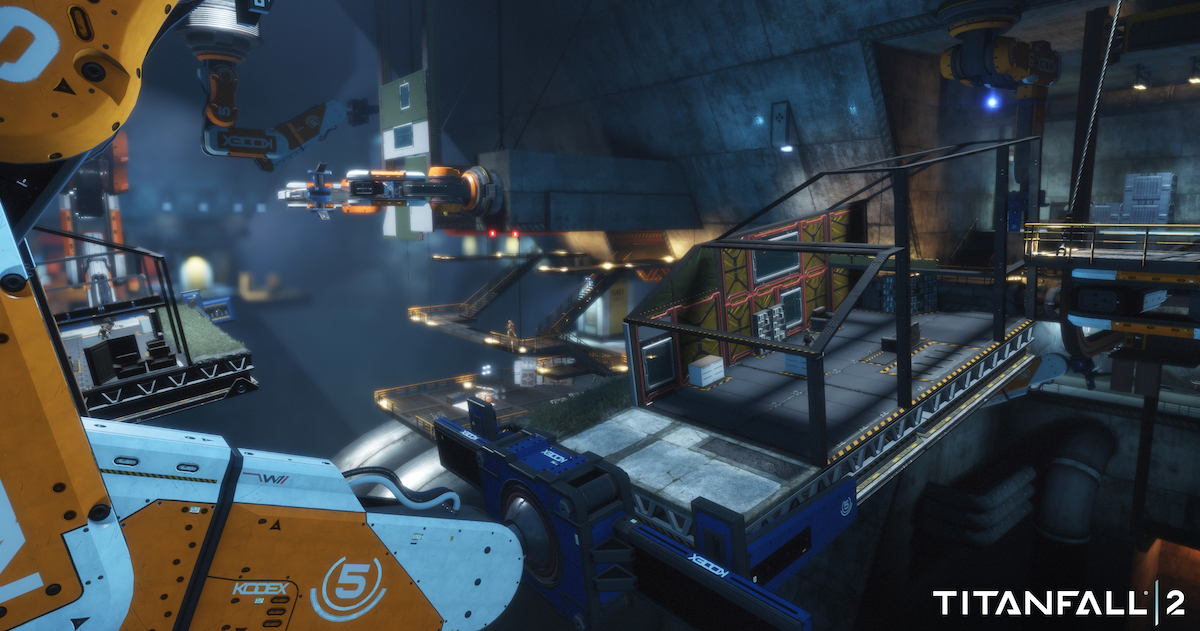
\includegraphics[width=\textwidth]{action_blocks_header}
\caption{Titanfall 2: Greybox-прототипы уровней, созданных по методу Action Blocks.
Скриншот из доклада Christopher Dionne на GDC 2018.
\textit{Источник: 80.lv / GDC Vault}}
\label{fig:action_blocks_header}
\end{figure}

\section{Процесс работы с Action Blocks}

\begin{tikzpicture}[
  node distance=0.8cm and 1.5cm,
  block/.style={
    rectangle, rounded corners=4pt,
    minimum width=3cm, minimum height=1.2cm,
    draw=titanblue, fill=titanblue!10,
    font=\small\bfseries, text=titandark, align=center
  },
  bigblock/.style={
    rectangle, rounded corners=4pt,
    minimum width=3.5cm, minimum height=1.4cm,
    draw=titanorange, fill=titanorange!10,
    font=\small\bfseries, text=titandark, align=center
  },
  arr/.style={-{Stealth[length=5pt]}, thick, titanblue!70}
]
  % Phase 1
  \node[block] (idea) {1. Идея\\(1--2 часа)};
  \node[block, right=of idea] (proto) {2. Прототип\\(2--5 дней)};
  \node[block, right=of proto] (play) {3. Плейтест\\(1 день)};
  \node[bigblock, right=of play] (eval) {4. Оценка\\Годится?};

  \draw[arr] (idea) -- (proto);
  \draw[arr] (proto) -- (play);
  \draw[arr] (play) -- (eval);

  % Branch
  \node[block, below=1cm of idea, fill=titanred!10, draw=titanred]
    (trash) {В корзину};
  \node[block, below=1cm of eval, fill=titangreen!10, draw=titangreen]
    (prod) {В продакшен};

  \draw[arr, titanred] (eval.south) -- ++(0,-0.5) -| (trash.north)
    node[midway, above, font=\scriptsize] {Нет};
  \draw[arr, titangreen] (eval.south) -- (prod.north)
    node[midway, right, font=\scriptsize] {Да};

  % Stats
  \node[below=2.5cm of proto, font=\small, text=titandark, text width=10cm, align=center] {
    \textbf{Статистика Titanfall 2:}
    100--200+ блоков создано за цикл разработки.\\
    Около 10--15\% прошли в финальную игру.
  };
\end{tikzpicture}

\subsection{Правила создания Action Block}

\begin{enumerate}[leftmargin=*]
  \item \textbf{Один дизайнер, одна идея.} Блок создаётся одним человеком.
    Никаких комитетов на этапе прототипа.
  \item \textbf{Placeholder всё.} Грейбокс-геометрия, временные анимации,
    заглушки вместо VFX. Цель~--- проверить \textit{fun}, не визуал.
  \item \textbf{Нет ограничений.} Дизайнер может пробовать любую механику,
    даже если она кажется безумной.
  \item \textbf{Нет привязанности.} Если блок не работает~--- его выбрасывают
    без сожалений.
  \item \textbf{Короткий цикл.} От идеи до плейтеста~--- максимум неделя.
\end{enumerate}

\begin{figure}[H]
\centering
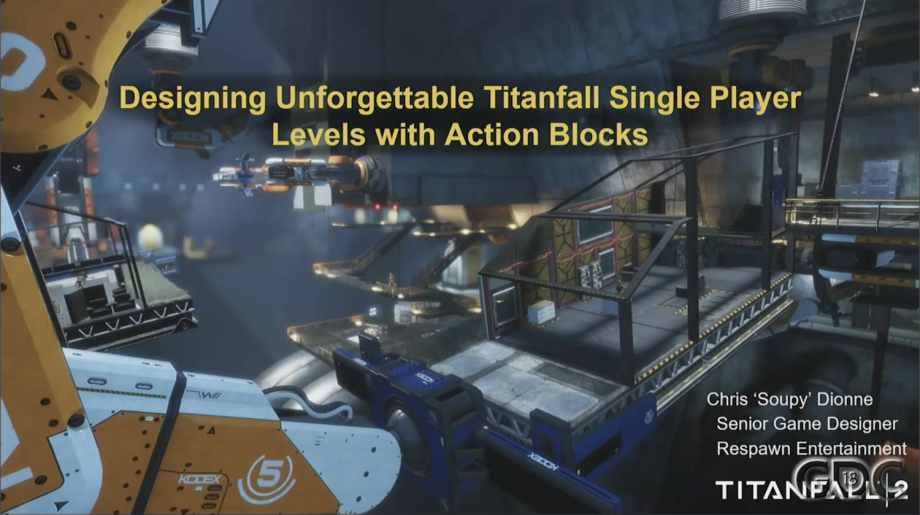
\includegraphics[width=0.48\textwidth]{action_blocks_1}
\hfill
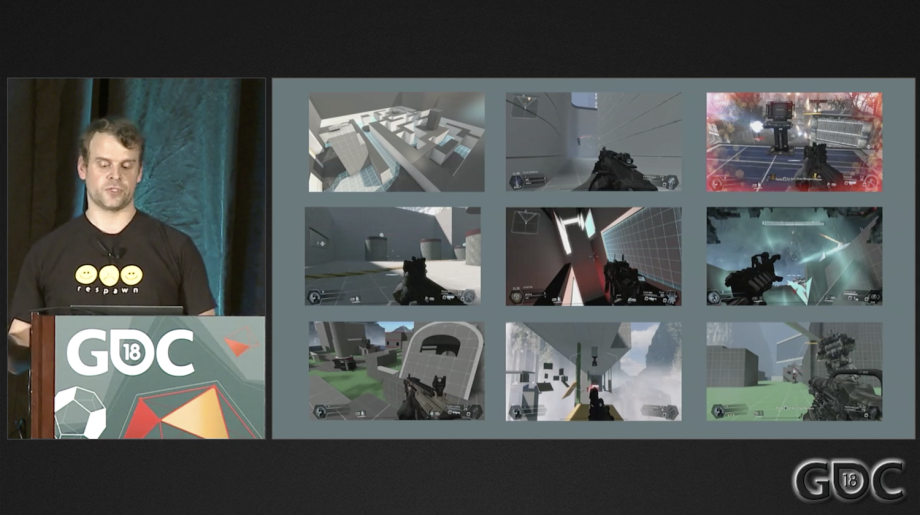
\includegraphics[width=0.48\textwidth]{action_blocks_2}
\caption{Примеры Action Blocks из разработки Titanfall 2: грейбокс-прототипы
отдельных геймплейных фрагментов. Каждый блок создан одним дизайнером
за несколько дней. \textit{Источник: 80.lv / GDC Vault}}
\label{fig:action_blocks_examples}
\end{figure}

\begin{example}{Пример: <<Effect and Cause>>}
Дизайнер Jake Keating взял мультиплеерную карту из первого Titanfall и
добавил на неё механику переключения между двумя состояниями
(прошлое/настоящее). Два уровня были <<стопками>> друг над другом.
Эта простая идея превратилась в один из самых знаменитых уровней
в истории FPS.
\end{example}

\section{Адаптация для маленькой команды}

\begin{tip}{Для инди-команд (1--5 человек)}
\begin{itemize}[leftmargin=*]
  \item Вместо 200 блоков делайте 10--20 за спринт
  \item Каждый блок~--- 1--3 дня, не больше
  \item Плейтест: друзья, семья, Discord-сообщество
  \item Фиксируйте видео каждого плейтеста
  \item Лучшие блоки = ядро ваших climax-арен
\end{itemize}
\end{tip}


% =============================================================================
% CHAPTER 3: ANATOMY OF AN ARENA
% =============================================================================
\chapter{Анатомия боевой арены}

\section{Что такое арена в контексте FPS}

\begin{principle}{Определение}
Арена~--- замкнутое или полузамкнутое пространство, спроектированное
для интенсивного боевого столкновения. Игрок входит, сражается с
волнами или группами врагов, и выходит (или продолжает уровень).
\end{principle}

Арена~--- это не просто комната с врагами. Это \textbf{боевая головоломка},
где геометрия, враги и ресурсы создают систему взаимодействий.

\section{Ключевые элементы арены}

\subsection{Петли (Loops)}

\begin{tikzpicture}[
  scale=0.9,
  room/.style={
    rectangle, rounded corners=2pt,
    minimum width=1.5cm, minimum height=1cm,
    draw=titandark, fill=titanlight,
    font=\scriptsize\bfseries
  },
  corridor/.style={thick, titandark},
  loopline/.style={very thick, dashed}
]
  % Simple arena with loops
  \node[font=\bfseries\color{titandark}, anchor=south] at (4,5.5) {Арена с двумя петлями};

  % Main arena space
  \draw[thick, fill=titanblue!8] (1,1) rectangle (7,5);
  \node[font=\small, text=titandark] at (4,4.5) {\textbf{Центральная зона}};

  % Cover objects
  \fill[titandark!30] (2.5,2.5) rectangle (3.2,3.2);
  \node[font=\tiny] at (2.85,2.85) {cover};
  \fill[titandark!30] (4.8,3.3) rectangle (5.5,4.0);
  \node[font=\tiny] at (5.15,3.65) {cover};

  % Entrance
  \draw[very thick, titangreen, -{Stealth}] (0,3) -- (1,3);
  \node[font=\scriptsize, titangreen, left] at (0,3) {Вход};

  % Exit
  \draw[very thick, titanred, -{Stealth}] (7,3) -- (8,3);
  \node[font=\scriptsize, titanred, right] at (8,3) {Выход};

  % Loop 1 (upper)
  \draw[loopline, polaritypos, -{Stealth}]
    (2,4.5) -- (2,5.5) -- (6,5.5) -- (6,4.5);
  \node[font=\scriptsize, polaritypos, above] at (4,5.5) {Петля A (верхний обход)};

  % Loop 2 (lower)
  \draw[loopline, polarityneg, -{Stealth}]
    (2,1.5) -- (2,0.5) -- (6,0.5) -- (6,1.5);
  \node[font=\scriptsize, polarityneg, below] at (4,0.5) {Петля B (нижний обход)};

  % Elevation marker
  \draw[thick, titanorange, -{Stealth}] (5.8,2) -- (5.8,4);
  \node[font=\scriptsize, titanorange, rotate=90, anchor=south] at (6.2,3)
    {Вертикаль};
\end{tikzpicture}

\begin{principle}{Принцип петель}
Петли позволяют игроку \textbf{маневрировать вокруг противников}, а не
отстреливаться от входа. Хорошая арена имеет минимум 2 петли, давая
выбор направления фланга.
\end{principle}

Основные типы петель:
\begin{itemize}[leftmargin=*]
  \item \textbf{Горизонтальные петли}~--- обходные пути на одном уровне
  \item \textbf{Вертикальные петли}~--- лестницы, лифты, wallrun-маршруты
  \item \textbf{Shortcuts}~--- однонаправленные проходы (спрыгнуть можно, вернуться нельзя)
\end{itemize}

\subsection{Укрытия (Cover)}

\begin{tikzpicture}[scale=0.85]
  % Title
  \node[font=\bfseries\color{titandark}] at (6,6.5) {Типы укрытий и их параметры};

  % Full cover
  \draw[thick, fill=titandark!40] (0.5,4) rectangle (2,5.5);
  \node[font=\scriptsize, text=white] at (1.25,4.75) {Full};
  \draw[thick, dashed, titanred] (0.5,5.5) -- (0.5,6) -- (-0.3,6);
  \node[font=\tiny, titanred] at (-0.3,6.3) {LOS blocked};

  % Half cover
  \draw[thick, fill=titandark!25] (4,4) rectangle (5.5,4.8);
  \node[font=\scriptsize] at (4.75,4.4) {Half};
  \draw[thick, dashed, titanorange] (4,4.8) -- (4,6);
  \node[font=\tiny, titanorange] at (4,6.3) {Head exposed};

  % Destructible cover
  \draw[thick, fill=titanorange!30, pattern=north east lines, pattern color=titanorange!40]
    (7.5,4) rectangle (9,5.2);
  \node[font=\scriptsize] at (8.25,4.6) {Destruct.};
  \node[font=\tiny, titanred] at (8.25,3.7) {Временное};

  % Pillar cover (360 degree)
  \draw[thick, fill=titandark!30] (11,4.5) circle (0.5);
  \node[font=\scriptsize] at (11,4.5) {Pillar};
  \draw[thick, dashed, titangreen] (11,4.5) circle (1);
  \node[font=\tiny, titangreen] at (11,3.2) {360\textdegree{} вращение};

  % Legend
  \node[font=\small, text=titandark, text width=12cm, align=left] at (6,2.5) {
    \textbf{Параметры укрытия:}\\
    \textbullet{} \textbf{Высота:} полное (full) / половинное (half) / отсутствует\\
    \textbullet{} \textbf{Ширина:} узкое (pillar) / широкое (wall)\\
    \textbullet{} \textbf{Прочность:} постоянное / разрушаемое / временное\\
    \textbullet{} \textbf{Facing:} одностороннее / многостороннее (pillar = 360\textdegree)
  };
\end{tikzpicture}

\begin{warning}{Анти-паттерн: Chest-High Walls}
В Action FPS с быстрым движением (wallrun, dash, double jump)
классические <<стены по грудь>> из Gears of War \textbf{не работают}.
Укрытия должны быть элементами \textbf{для прохождения через них},
а не для прятания за ними. Колонна, от которой можно оттолкнуться
wallrun-ом~--- лучше, чем стена, за которой можно сидеть.
\end{warning}

\subsection{Линии видимости (Sightlines)}

\begin{tikzpicture}[scale=0.8]
  \node[font=\bfseries\color{titandark}] at (6,7) {Управление линиями видимости};

  % Arena outline
  \draw[thick, fill=titanblue!5] (0,0) rectangle (12,6);

  % Player position
  \fill[titangreen] (1,3) circle (0.3);
  \node[font=\scriptsize, titangreen, left] at (0.5,3) {Player};

  % Enemy positions
  \fill[titanred] (10,5) circle (0.2);
  \fill[titanred] (8,1) circle (0.2);
  \fill[titanred] (11,3) circle (0.2);

  % Cover blocks
  \fill[titandark!40] (4,2) rectangle (5,4);
  \fill[titandark!40] (7,3.5) rectangle (8,5);

  % Sightline 1 - blocked
  \draw[thick, dashed, titanred!50] (1,3) -- (4,3);
  \node[font=\tiny, titanred] at (2.5,3.3) {Blocked};
  \draw[thick, titanred, -{Stealth}] (5,3) -- (11,3);

  % Sightline 2 - open
  \draw[thick, titangreen, -{Stealth}] (1,3) -- (8,1);
  \node[font=\tiny, titangreen] at (4.5,1.7) {Open LOS};

  % Sightline 3 - partial
  \draw[thick, titanorange, -{Stealth}] (1,3) -- (7,5);
  \node[font=\tiny, titanorange] at (3,4.5) {Partial LOS};

  % Annotations
  \node[font=\small, text=titandark, text width=11cm, align=left] at (6,-1.5) {
    \textbf{Правила:}
    Ни одна позиция не должна давать обзор всей арены.
    Каждая линия видимости = risk/reward для игрока.
    Длинные прямые коридоры создают <<снайперские зоны>>,
    перпендикулярные стены создают <<углы столкновений>>.
  };
\end{tikzpicture}

\subsection{Вертикальность (Verticality)}

\begin{principle}{Принцип вертикальности}
Вертикальность увеличивает количество игровых решений и
\textbf{геймплей на квадратный метр}. Полностью плоская карта
на 32 игрока может быть 400$\times$400~м, но добавив 2 уровня
вертикальности, можно уместить тот же геймплей в 200$\times$200~м.
\end{principle}

В контексте Titanfall~2 и Action FPS вертикальность включает:
\begin{itemize}[leftmargin=*]
  \item \textbf{Этажи и балконы}~--- классическая вертикаль
  \item \textbf{Wallrun-маршруты}~--- вертикаль через движение
  \item \textbf{Прыжковые площадки}~--- launch pads, гейзеры, взрывные бочки
  \item \textbf{Высотные преимущества}~--- high ground = лучший обзор, но
    и большая уязвимость (игрок виден со многих точек)
\end{itemize}

\begin{tikzpicture}[scale=0.75]
  \node[font=\bfseries\color{titandark}] at (5,9.5) {Вертикальный разрез арены};

  % Ground level
  \fill[titanblue!10] (0,0) rectangle (10,2);
  \draw[thick] (0,0) -- (10,0);
  \draw[thick] (0,2) -- (4,2) (6,2) -- (10,2);
  \node[font=\scriptsize, titanblue] at (5,1) {Уровень 1: Основной};

  % Mid level
  \fill[titanorange!10] (0,3) rectangle (4,5);
  \fill[titanorange!10] (6,3) rectangle (10,5);
  \draw[thick] (0,3) -- (4,3) (6,3) -- (10,3);
  \draw[thick] (0,5) -- (3,5) (7,5) -- (10,5);
  \node[font=\scriptsize, titanorange] at (2,4) {Уровень 2};
  \node[font=\scriptsize, titanorange] at (8,4) {Уровень 2};

  % High level
  \fill[titanred!10] (1,6) rectangle (3.5,7.5);
  \fill[titanred!10] (7,6) rectangle (9.5,7.5);
  \draw[thick] (1,6) -- (3.5,6);
  \draw[thick] (1,7.5) -- (3.5,7.5);
  \draw[thick] (7,6) -- (9.5,6);
  \draw[thick] (7,7.5) -- (9.5,7.5);
  \node[font=\scriptsize, titanred] at (2.25,6.75) {Уровень 3};
  \node[font=\scriptsize, titanred] at (8.25,6.75) {Уровень 3};

  % Wallrun surface
  \draw[very thick, titancyan] (4.2,2) -- (4.2,5.5);
  \node[font=\tiny, titancyan, rotate=90, anchor=south] at (3.8,3.5) {Wallrun};

  % Jump arc
  \draw[thick, dashed, titangreen, -{Stealth}]
    (3.5,5) to[out=30,in=150] (7,5);
  \node[font=\tiny, titangreen, above] at (5.25,5.8) {Double Jump};

  % Drop down
  \draw[thick, titanorange, -{Stealth}] (9,6) -- (9,3.2);
  \node[font=\tiny, titanorange, right] at (9.1,4.5) {Drop};

  % Labels
  \node[font=\scriptsize, titandark] at (5,2.5) {\textit{Открытый атриум}};
\end{tikzpicture}


\section{Архетипы арен}

\subsection{Skate Park (DOOM Eternal)}

\begin{tikzpicture}[scale=0.7]
  \node[font=\bfseries\color{titandark}] at (5,7.5) {<<Skate Park>> --- арена DOOM Eternal};

  % Central arena
  \draw[thick, fill=titanblue!8] (0,0) -- (10,0) -- (10,7) -- (0,7) -- cycle;

  % Circular flow arrows
  \draw[very thick, titanorange, -{Stealth}]
    (1,1) -- (9,1) -- (9,6) -- (1,6) -- cycle;
  \node[font=\small, titanorange] at (5,3.5) {\textbf{Circular Flow}};

  % Platforms
  \fill[titandark!20] (2,2.5) rectangle (4,4.5);
  \node[font=\tiny] at (3,3.5) {Platform};

  \fill[titandark!20] (6,3) rectangle (8,5);
  \node[font=\tiny] at (7,4) {Platform};

  % Jump pads
  \fill[titangreen] (1,1) circle (0.2);
  \fill[titangreen] (9,1) circle (0.2);
  \fill[titangreen] (5,6) circle (0.2);
  \node[font=\tiny, titangreen] at (1,0.5) {Pad};
  \node[font=\tiny, titangreen] at (9,0.5) {Pad};

  % Note
  \node[font=\small, text=titandark, text width=10cm, align=left] at (5,-1.2) {
    Ключевая идея: игрок \textbf{никогда не останавливается}. Арена
    спроектирована как трек для скейтборда~--- движение по кругу,
    прыжковые панели поддерживают momentum.
  };
\end{tikzpicture}

\subsection{Jungle Gym (DOOM Eternal)}

Многоэтажная арена с отдельными <<этажами>> и вертикальными
переходами. Игрок перемещается между уровнями, используя лифты,
прыжковые площадки и monkey bars.

\subsection{Canyon (линейная с вертикалью)}

Узкое вытянутое пространство с высокими стенами. Wallrun и
вертикальное движение~--- основной способ перемещения. Подходит для
chase-последовательностей.

\begin{figure}[H]
\centering
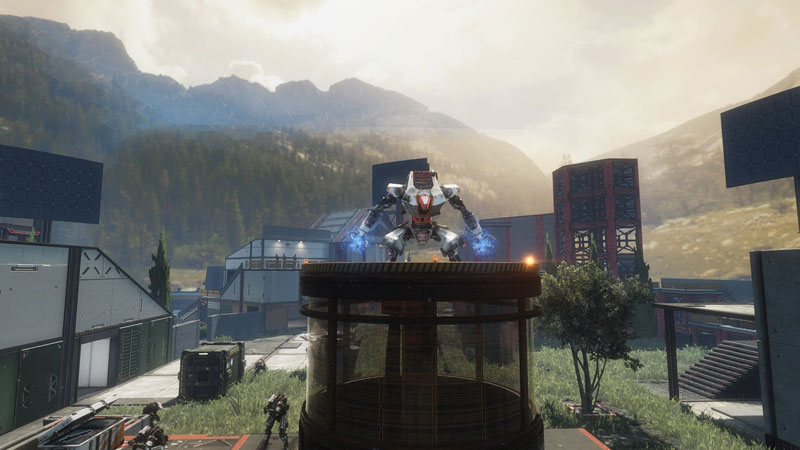
\includegraphics[width=0.48\textwidth]{into_abyss_4}
\hfill
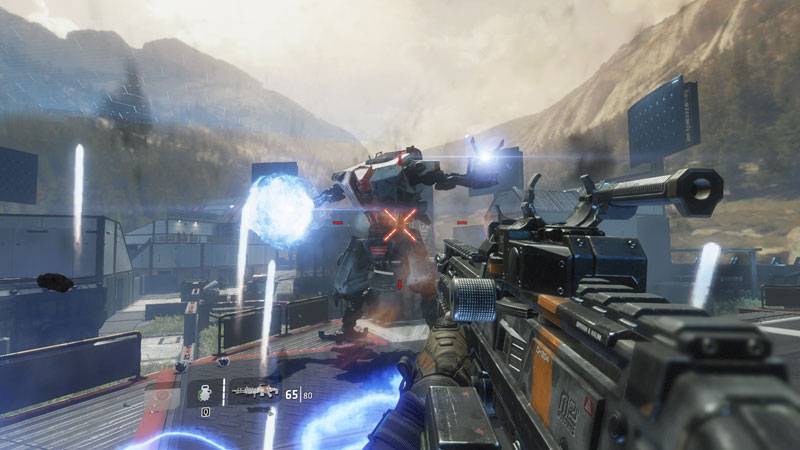
\includegraphics[width=0.48\textwidth]{into_abyss_5}
\caption{Примеры боевых арен из <<Into the Abyss>>: открытые пространства
с вертикальностью, множеством путей и динамической геометрией.
\textit{Источник: davidshaver.net}}
\label{fig:into_abyss_arenas}
\end{figure}

\subsection{Hub \& Spokes (Titanfall 2 style)}

\begin{tikzpicture}[scale=0.8]
  \node[font=\bfseries\color{titandark}] at (5,7) {<<Hub \& Spokes>> --- структура уровня TF2};

  % Central hub
  \draw[thick, fill=titanorange!15] (5,3.5) circle (1.5);
  \node[font=\bfseries, titanorange] at (5,3.5) {HUB};

  % Spokes - POI A
  \draw[thick, titangreen, -{Stealth}] (5,3.5) ++(30:1.5) -- ++(30:2);
  \node[font=\scriptsize, titangreen] at ($(5,3.5)+(30:4)$) {POI A};
  \fill[titangreen!30] ($(5,3.5)+(30:3.5)$) circle (0.4);
  % Climax Arena
  \draw[thick, titanred, -{Stealth}] (5,3.5) ++(90:1.5) -- ++(90:2);
  \node[font=\scriptsize, titanred] at ($(5,3.5)+(90:4)$) {Climax Arena};
  \fill[titanred!30] ($(5,3.5)+(90:3.5)$) circle (0.4);
  % POI B
  \draw[thick, titangreen, -{Stealth}] (5,3.5) ++(150:1.5) -- ++(150:2);
  \node[font=\scriptsize, titangreen] at ($(5,3.5)+(150:4)$) {POI B};
  \fill[titangreen!30] ($(5,3.5)+(150:3.5)$) circle (0.4);
  % POI C
  \draw[thick, titangreen, -{Stealth}] (5,3.5) ++(210:1.5) -- ++(210:2);
  \node[font=\scriptsize, titangreen] at ($(5,3.5)+(210:4)$) {POI C};
  \fill[titangreen!30] ($(5,3.5)+(210:3.5)$) circle (0.4);
  % Вход
  \draw[thick, titanblue, -{Stealth}] (5,3.5) ++(270:1.5) -- ++(270:2);
  \node[font=\scriptsize, titanblue] at ($(5,3.5)+(270:4)$) {Вход};
  \fill[titanblue!30] ($(5,3.5)+(270:3.5)$) circle (0.4);
  % POI D
  \draw[thick, titangreen, -{Stealth}] (5,3.5) ++(330:1.5) -- ++(330:2);
  \node[font=\scriptsize, titangreen] at ($(5,3.5)+(330:4)$) {POI D};
  \fill[titangreen!30] ($(5,3.5)+(330:3.5)$) circle (0.4);

  \node[font=\small, text=titandark, text width=10cm, align=center] at (5,-0.5) {
    Центральная зона (Hub) соединяет все точки интереса.\\
    Игрок свободно выбирает порядок посещения POI.\\
    Climax Arena~--- обязательный финал.
  };
\end{tikzpicture}


% =============================================================================
% CHAPTER 4: ENCOUNTER DESIGN
% =============================================================================
\chapter{Дизайн боевых столкновений (Encounter Design)}

\section{Структура энкаунтера}

Каждое боевое столкновение~--- это мини-история с началом, серединой
и кульминацией.

\begin{tikzpicture}[
  scale=0.9,
  phase/.style={
    rectangle, rounded corners=3pt,
    minimum width=3.5cm, minimum height=1.5cm,
    draw=#1, fill=#1!10,
    font=\small\bfseries, text=titandark, align=center
  }
]
  \node[phase=titangreen] (begin) at (0,0) {НАЧАЛО\\Survey \& Plan};
  \node[phase=titanorange] (middle) at (5.5,0) {СЕРЕДИНА\\Fight \& Adapt};
  \node[phase=titanred] (climax) at (11,0) {КУЛЬМИНАЦИЯ\\Peak \& Resolve};

  \draw[very thick, -{Stealth}, titanblue] (begin) -- (middle);
  \draw[very thick, -{Stealth}, titanblue] (middle) -- (climax);

  % Details below
  \node[text width=3.3cm, align=center, font=\tiny, below=4pt of begin] {
    Игрок осматривает арену,\\
    видит врагов, планирует\\
    первую атаку
  };
  \node[text width=3.3cm, align=center, font=\tiny, below=4pt of middle] {
    Бой, волны, адаптация\\
    к новым угрозам,\\
    скриптовые события
  };
  \node[text width=3.3cm, align=center, font=\tiny, below=4pt of climax] {
    Максимальная интенсивность,\\
    boss/elite wave,\\
    разрешение
  };
\end{tikzpicture}

\section{Три метода начала энкаунтера}

\subsection{Метод 1: Засада игрока (Player Ambush)}

Враги начинают в расслабленном состоянии. Игрок видит их с входа и
\textbf{сам решает}, когда начать бой. Первый выстрел~--- за игроком.

\begin{example}{Пример: Titanfall 2 <<Effect and Cause>>, Encounter 1}
11 врагов (4 в первой комнате, 7 во второй) существуют только в
<<прошлом>>. Игрок может спокойно осмотреть арену из <<настоящего>>,
спланировать атаку, и переключиться в прошлое для боя.
Отступление назад в <<настоящее>>~--- всегда доступно.
\end{example}

\subsection{Метод 2: Засада на игрока (Enemy Ambush)}

Пустая арена. Враги появляются, когда игрок пересекает невидимый
триггер в середине пространства. Работает \textbf{один раз}~--- повторное
использование ведёт к trial-and-error фрустрации.

\begin{warning}{Ограничение}
Не используйте засаду на игрока чаще одного раза за уровень.
При повторении игрок начинает ожидать подвох и теряет доверие к
пространству. Сложность засады должна быть \textbf{ниже средней},
чтобы компенсировать отсутствие подготовки.
\end{warning}

\subsection{Метод 3: Vista с односторонним входом}

Игрок видит врагов с возвышенности через стекло или с большого
расстояния. Он \textbf{не может атаковать} с этой позиции. Затем
спрыгивает / проходит через шлюз~--- и назад пути нет.

Этот метод создаёт максимальное напряжение: <<Я вижу, что меня ждёт,
но войдя~--- не смогу вернуться>>.

\section{Палитра врагов}

\begin{table}[H]
\centering
\caption{Рекомендации по количеству типов врагов в энкаунтере}
\begin{tabularx}{\textwidth}{@{}cXX@{}}
\toprule
\textbf{Типов} & \textbf{Функция} & \textbf{Опыт игрока} \\
\midrule
1 & Туториал/отдых & Фокус на одном типе \\
2 & Стандартный энкаунтер & Типы взаимодействуют осмысленно \\
3 & Сложный/хаотичный & Читаемость снижается \\
4+ & Boss fight, финал уровня & Только для опытных игроков \\
\bottomrule
\end{tabularx}
\end{table}

\begin{principle}{Принцип <<триады врагов>>}
Хорошая палитра врагов для одного энкаунтера:
\textbf{Aggressor} (бросается в ближний бой) +
\textbf{Anchor} (стреляет с позиции) +
\textbf{Disruptor} (заставляет менять позицию:
гранатомётчик, щитоносец, снайпер).
\end{principle}

\begin{tikzpicture}[
  role/.style={
    circle, minimum size=2.5cm,
    draw=#1, fill=#1!10,
    font=\small\bfseries, text=titandark, align=center
  }
]
  \node[role=titanred] (aggr) at (0,0) {Aggressor\\{\scriptsize Rush / Melee}};
  \node[role=titanblue] (anchor) at (5,0) {Anchor\\{\scriptsize Hold / Shoot}};
  \node[role=titanorange] (disrupt) at (2.5,3) {Disruptor\\{\scriptsize Force Move}};

  \draw[very thick, titandark!50] (aggr) -- (anchor) -- (disrupt) -- (aggr);

  \node[font=\tiny, text=titandark, below=2pt] at (2.5,-0.3) {Давит на позицию};
  \node[font=\tiny, text=titandark, rotate=55, above left=2pt] at (1,1.5) {Давит на время};
  \node[font=\tiny, text=titandark, rotate=-55, above right=2pt] at (4,1.5) {Давит на спэйс};
\end{tikzpicture}


\section{Прогрессия энкаунтеров в <<Effect and Cause>>}

\begin{tikzpicture}[scale=0.85]
  \begin{axis}[
    width=14cm, height=6cm,
    xlabel={Прогресс уровня},
    ylabel={Сложность / Напряжение},
    xmin=0, xmax=100,
    ymin=0, ymax=10,
    xtick={15,50,85},
    xticklabels={Encounter 1, Encounter 2, Encounter 3},
    ytick={2,5,8},
    yticklabels={Низкая, Средняя, Высокая},
    grid=major,
    grid style={titanlight},
    axis lines=left,
    title={\textbf{Кривая сложности <<Effect and Cause>>}},
    title style={font=\bfseries\color{titandark}},
    xlabel style={font=\small},
    ylabel style={font=\small}
  ]
    % Intensity curve
    \addplot[very thick, titanblue, smooth] coordinates {
      (0,1) (5,1.5) (10,2) (15,3) (20,2) (25,1.5) (30,2)
      (35,3) (40,4) (45,5) (50,6) (55,4) (60,3.5) (65,4)
      (70,5) (75,6) (80,7) (85,8.5) (90,9) (95,7) (100,4)
    };

    % Annotations
    \node[font=\tiny, titangreen, fill=white, inner sep=1pt] at (axis cs:15,3.5) {Safe learning};
    \node[font=\tiny, titanorange, fill=white, inner sep=1pt] at (axis cs:50,6.5) {Dual-timeline};
    \node[font=\tiny, titanred, fill=white, inner sep=1pt] at (axis cs:87,9.3) {Full mastery};

    % Rest zones
    \addplot[fill=titangreen!20, draw=none, forget plot] coordinates {
      (20,0) (20,2) (30,2) (30,0)
    } -- cycle;
    \addplot[fill=titangreen!20, draw=none, forget plot] coordinates {
      (55,0) (55,4) (65,3.5) (65,0)
    } -- cycle;
  \end{axis}
  \node[font=\tiny, titangreen] at (3.2,0.5) {Rest};
  \node[font=\tiny, titangreen] at (7.7,0.5) {Rest};
\end{tikzpicture}

\subsection{Encounter 1: Безопасное обучение}

\begin{itemize}[leftmargin=*]
  \item 11 врагов (4 + 7), только в <<прошлом>>
  \item Игрок может экспериментировать без наказания
  \item Цель: понять механику переключения времени
  \item Низкое давление, много пространства для отступления
\end{itemize}

\subsection{Encounter 2: Тактическая сложность}

\begin{itemize}[leftmargin=*]
  \item Большая комната с вертикальностью (балконы, лестницы, лифты)
  \item 11 солдат (9 обычных + 2 тяжёлых со щитами) в прошлом
  \item 3 робота + 4 prowler-а в настоящем
  \item Первый раз, когда \textbf{оба} времени опасны
  \item Игрок должен приоритизировать угрозы между таймлайнами
\end{itemize}

\subsection{Encounter 3: Финальный тест мастерства}

\begin{itemize}[leftmargin=*]
  \item Два вертикально связанных пространства
  \item 12 солдат + 3 робота в прошлом; 8+ prowler-ов в настоящем
  \item Минимум ограничений~--- игрок сам выбирает стратегию
  \item Множество путей, zip-lines, фланговые маршруты
  \item Максимальное skill expression
\end{itemize}


% =============================================================================
% CHAPTER 5: PACING
% =============================================================================
\chapter{Пейсинг --- ритм уровня}

\section{Кривая интенсивности}

Пейсинг~--- это \textbf{управление эмоциональной интенсивностью} игрока
на протяжении уровня. Хороший пейсинг чередует пики напряжения
с моментами отдыха.

\begin{tikzpicture}
  \begin{axis}[
    width=14cm, height=7cm,
    xlabel={Время прохождения уровня (мин)},
    ylabel={Интенсивность},
    xmin=0, xmax=15,
    ymin=0, ymax=10,
    ytick={0,2,4,6,8,10},
    yticklabels={, Exploration, Light Combat, Combat, Intense, CLIMAX},
    grid=major,
    grid style={titanlight},
    axis lines=left,
    title={\textbf{Идеальная кривая интенсивности для 15-минутного уровня}},
    title style={font=\bfseries\color{titandark}}
  ]
    % Ideal curve
    \addplot[very thick, titanblue, smooth] coordinates {
      (0,1) (0.5,2) (1,3)
      (2,5) (2.5,6) (3,4)
      (3.5,3) (4,2)
      (4.5,3) (5,4) (5.5,5)
      (6,6) (6.5,7) (7,5)
      (7.5,3) (8,2.5) (8.5,2)
      (9,3) (9.5,4) (10,5)
      (10.5,6) (11,7) (11.5,8)
      (12,8.5) (12.5,9) (13,9.5)
      (13.5,10) (14,8) (14.5,5) (15,3)
    };

    % Phase labels
    \draw[thick, titangreen, dashed] (axis cs:0,0) -- (axis cs:0,10);
    \draw[thick, titanorange, dashed] (axis cs:4,0) -- (axis cs:4,10);
    \draw[thick, titanred, dashed] (axis cs:9,0) -- (axis cs:9,10);

    \node[font=\scriptsize\bfseries, titangreen, rotate=90, anchor=south]
      at (axis cs:2,9) {ACT 1: Introduction};
    \node[font=\scriptsize\bfseries, titanorange, rotate=90, anchor=south]
      at (axis cs:6.5,9) {ACT 2: Development};
    \node[font=\scriptsize\bfseries, titanred, rotate=90, anchor=south]
      at (axis cs:12,9) {ACT 3: Climax};

    % Rest zones highlighted
    \addplot[fill=titangreen!15, draw=none, forget plot] coordinates {
      (3,0) (3,4) (4.5,3) (4.5,0)
    } -- cycle;
    \addplot[fill=titangreen!15, draw=none, forget plot] coordinates {
      (7,0) (7,5) (9,2) (9,0)
    } -- cycle;
  \end{axis}
\end{tikzpicture}

\section{Правило <<вдоха и выдоха>>}

\begin{principle}{Дыхание уровня (Breathing)}
После каждого интенсивного боя должна следовать зона \textbf{отдыха}:
traversal, exploration, лёгкая загадка, нарративный момент. Это:
\begin{itemize}
  \item Даёт игроку время осмыслить произошедшее
  \item Создаёт контраст, усиливающий следующий бой
  \item Предотвращает <<combat fatigue>>~--- утомление от непрерывного боя
\end{itemize}
\end{principle}

\begin{table}[H]
\centering
\caption{Чередование интенсивности для 15-минутного уровня}
\begin{tabularx}{\textwidth}{@{}clXc@{}}
\toprule
\textbf{Мин} & \textbf{Сегмент} & \textbf{Описание} & \textbf{Интенс.} \\
\midrule
0--1 & Вход & Exploration, ориентация, атмосфера & 2/10 \\
1--3 & Бой 1 & Первый энкаунтер, введение механики уровня & 5/10 \\
3--4.5 & Отдых & Traversal, лёгкая загадка, ресурсы & 2/10 \\
4.5--7 & Бой 2 & Развитие механики, новые враги & 7/10 \\
7--9 & Отдых & Нарративный момент, vista, preparation & 2/10 \\
9--13.5 & Climax & Финальная арена, все механики вместе & 9/10 \\
13.5--15 & Denouement & Победа, награда, переход & 3/10 \\
\bottomrule
\end{tabularx}
\end{table}

\section{Правило <<никогда дважды одно и то же>>}

\begin{principle}{Правило Titanfall 2}
Каждый <<вдох>> должен быть \textbf{другого типа}:
если первый отдых~--- traversal, то второй~--- нарративный момент.
Каждый <<выдох>> (бой) должен менять \textbf{правила игры}:
если первый бой~--- на открытой арене, то второй~--- в тесных
коридорах или с новым типом врага.
\end{principle}


% =============================================================================
% CHAPTER 6: MOVEMENT & TRAVERSAL
% =============================================================================
\chapter{Движение и траверсал}

\section{Движение как геймплей}

В Titanfall~2 движение~--- не способ добраться из точки A в точку B,
а \textbf{самостоятельная механика} с собственной системой мастерства.

\begin{principle}{Momentum-based design}
Уровень должен \textbf{награждать движение}. Остановка = опасность.
Wallrun увеличивает скорость со временем, что поощряет цепочки
wall-run-ов и создаёт естественный <<flow state>>.
\end{principle}

\section{Типы траверсальных элементов}

\begin{table}[H]
\centering
\caption{Траверсальные элементы и их роль в уровне}
\begin{tabularx}{\textwidth}{@{}lXcc@{}}
\toprule
\textbf{Элемент} & \textbf{Роль в дизайне} & \textbf{Скорость} & \textbf{Skill} \\
\midrule
Wallrun surface & Основной вертикальный маршрут & Высокая & Средний \\
Double jump gap & Горизонтальное препятствие & Средняя & Низкий \\
Slide ramp & Ускоритель + укрытие & Высокая & Низкий \\
Grapple point & Быстрое вертикальное перемещение & Очень выс. & Высокий \\
Launch pad & Принудительное перемещение & Контрол. & Низкий \\
Zip-line & Предсказуемый маршрут (уязвим) & Средняя & Низкий \\
Dash через пропасть & Точный timing + direction & Высокая & Высокий \\
\bottomrule
\end{tabularx}
\end{table}

\section{Дизайн traversal-секций}

\begin{tikzpicture}[scale=0.75]
  \node[font=\bfseries\color{titandark}] at (7,9) {Traversal-секция: цепочка wallrun-ов};

  % Platforms and walls
  \fill[titanblue!15] (0,0) rectangle (3,1);
  \node[font=\scriptsize] at (1.5,0.5) {Start Platform};

  % Wall 1
  \fill[titancyan!30] (3.5,0.5) rectangle (4,4);
  \node[font=\tiny, rotate=90] at (3.75,2.25) {Wall 1};

  % Wall 2
  \fill[titancyan!30] (6,2) rectangle (6.5,6);
  \node[font=\tiny, rotate=90] at (6.25,4) {Wall 2};

  % Wall 3
  \fill[titancyan!30] (8.5,3) rectangle (9,7);
  \node[font=\tiny, rotate=90] at (8.75,5) {Wall 3};

  % End platform
  \fill[titanblue!15] (11,6) rectangle (14,7);
  \node[font=\scriptsize] at (12.5,6.5) {End Platform};

  % Player path
  \draw[very thick, titanorange, -{Stealth}, dashed]
    (2.5,1) to[out=20,in=200] (3.5,2) % jump to wall 1
    -- (3.5,3.5) % wallrun up
    to[out=30,in=210] (6,3.5) % jump to wall 2
    -- (6,5.5) % wallrun up
    to[out=30,in=210] (8.5,5) % jump to wall 3
    -- (8.5,6.5) % wallrun up
    to[out=30,in=180] (11,6.5); % land

  % Danger zone
  \fill[titanred!15] (0,-1) rectangle (14,0);
  \node[font=\scriptsize, titanred] at (7,-0.5) {ОПАСНАЯ ЗОНА (токсичная жидкость, пропасть)};

  % Momentum arrows
  \draw[thick, titangreen, -{Stealth}] (1,1.3) -- (3,1.3);
  \node[font=\tiny, titangreen, above] at (2,1.3) {momentum};
\end{tikzpicture}

\begin{tip}{Золотое правило traversal}
Если игрок может пройти traversal-секцию с первой попытки, но
\textbf{быстрее и стильнее} с мастерством~--- дизайн правильный.
Если игрок \textbf{не может пройти} без точного знания маршрута~--- дизайн
провальный. Traversal должен быть \textbf{читаемым с первого взгляда}.
\end{tip}


% =============================================================================
% CHAPTER 7: SCRIPTED MOMENTS
% =============================================================================
\chapter{Скриптовые моменты и Set-Pieces}

\section{Что такое set-piece}

Set-piece~--- это \textbf{уникальное, скриптованное событие}, которое
происходит в определённый момент уровня и создаёт запоминающийся
опыт. Это может быть:

\begin{itemize}[leftmargin=*]
  \item Обрушение здания во время боя
  \item Внезапная смена масштаба (пеший бой $\to$ Титан)
  \item Головоломка, использующая уникальную механику уровня
  \item Визуально впечатляющий момент (vista, взрыв, панорама)
\end{itemize}

\section{Принципы скриптовых моментов}

\subsection{Player Agency First}

\begin{principle}{Принцип агентности}
Скриптовый момент должен \textbf{ощущаться как действие игрока},
а не как кат-сцена. Если здание падает~--- пусть оно падает,
пока игрок \textbf{бежит по нему}. Если враг взрывается~--- пусть это
результат действия игрока (например, выстрел в слабое место).
\end{principle}

\subsection{Timing и триггеры}

\begin{tikzpicture}[
  node distance=0.6cm,
  trig/.style={
    rectangle, rounded corners=2pt,
    minimum width=2.8cm, minimum height=0.9cm,
    draw=titanorange, fill=titanorange!10,
    font=\scriptsize\bfseries, align=center
  },
  event/.style={
    rectangle, rounded corners=2pt,
    minimum width=2.8cm, minimum height=0.9cm,
    draw=titanblue, fill=titanblue!10,
    font=\scriptsize\bfseries, align=center
  },
  arr/.style={-{Stealth[length=4pt]}, thick}
]
  \node[trig] (t1) at (0,0) {Trigger:\\Объём (Volume)};
  \node[trig] (t2) at (0,-1.5) {Trigger:\\Kill Count};
  \node[trig] (t3) at (0,-3) {Trigger:\\Таймер};
  \node[trig] (t4) at (0,-4.5) {Trigger:\\Взаимодействие};

  \node[event] (e1) at (5,0) {Spawn Wave};
  \node[event] (e2) at (5,-1.5) {Env. Change};
  \node[event] (e3) at (5,-3) {Dialogue};
  \node[event] (e4) at (5,-4.5) {Set-Piece};

  \draw[arr] (t1) -- (e1);
  \draw[arr] (t2) -- (e2);
  \draw[arr] (t3) -- (e3);
  \draw[arr] (t4) -- (e4);

  \node[font=\bfseries\color{titandark}, above=0.3cm of t1, anchor=south] {Триггеры};
  \node[font=\bfseries\color{titandark}, above=0.3cm of e1, anchor=south] {События};
\end{tikzpicture}

\subsection{Примеры set-pieces из Titanfall 2}

\begin{example}{<<Into the Abyss>> --- Фабрика}
Игрок перемещается по работающей фабрике с движущимися
конвейерами, прессами и роботизированными руками. Геометрия
уровня \textbf{постоянно движется}, создавая динамические
препятствия и укрытия. Это не скрипт~--- это системная механика,
встроенная в уровень.
\end{example}

\begin{figure}[H]
\centering
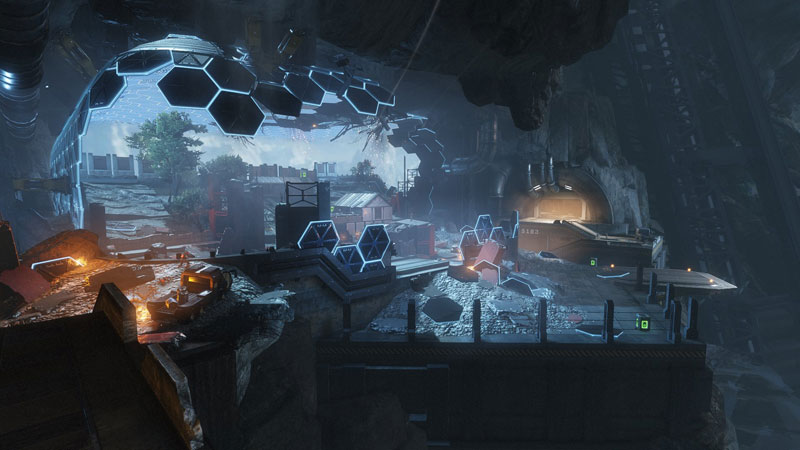
\includegraphics[width=0.48\textwidth]{into_abyss_0}
\hfill
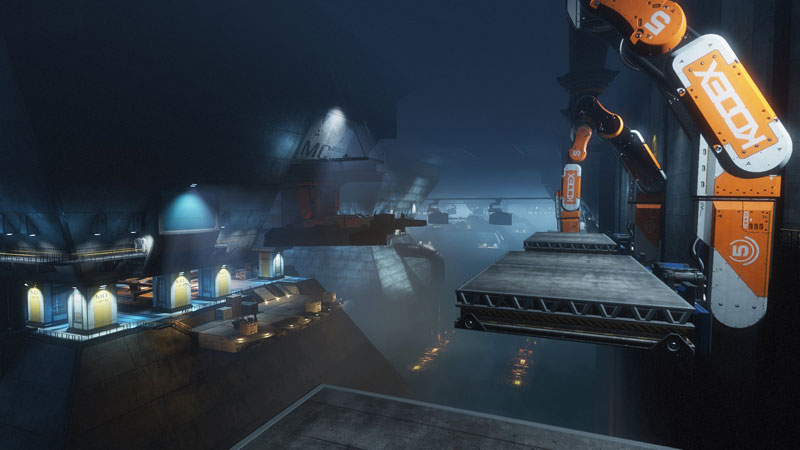
\includegraphics[width=0.48\textwidth]{into_abyss_1}\\[4pt]
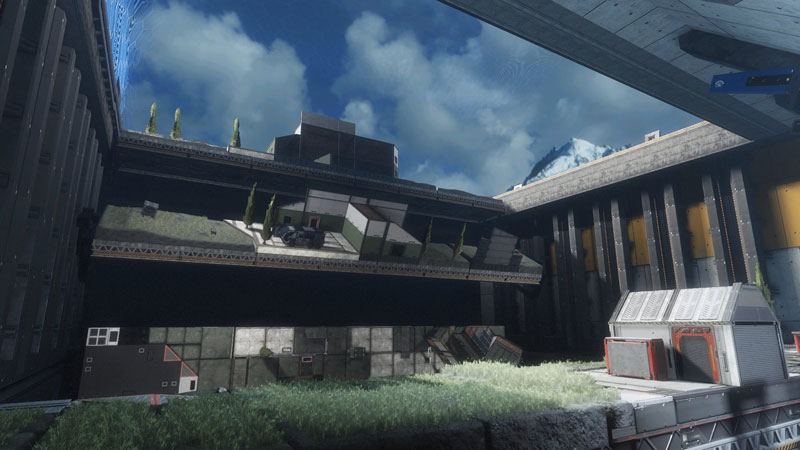
\includegraphics[width=0.48\textwidth]{into_abyss_2}
\hfill
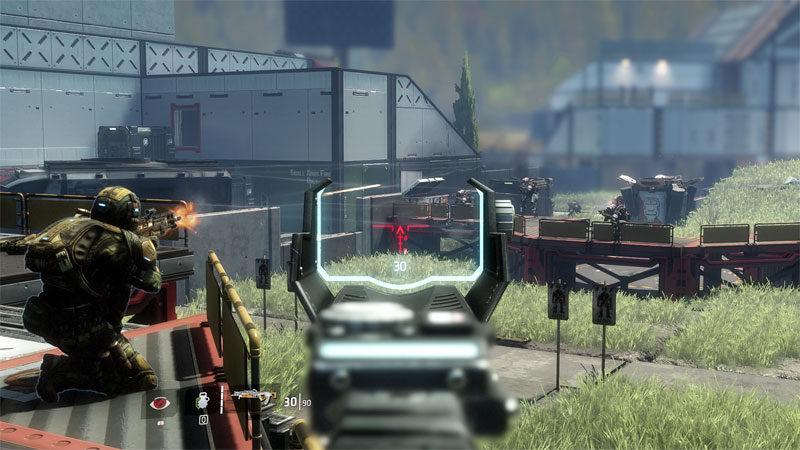
\includegraphics[width=0.48\textwidth]{into_abyss_3}
\caption{<<Into the Abyss>> (Titanfall 2)~--- кадры из готового уровня.
Фабрика World Foundry с движущейся геометрией, Simulation Dome и
масштабные боевые арены. Дизайн: David Shaver.
\textit{Источник: davidshaver.net}}
\label{fig:into_abyss}
\end{figure}

\begin{example}{<<Effect and Cause>> --- Переключение времени}
Игрок переключается между двумя состояниями одной локации.
В <<прошлом>>~--- работающий объект с солдатами.
В <<настоящем>>~--- разрушенные руины с роботами и тварями.
Стена в настоящем~--- проход в прошлом. Пол в прошлом~---
пропасть в настоящем. Две карты \textbf{стопкой друг над другом}.
\end{example}

\begin{example}{<<The Beacon>> --- Arc Tool}
Игрок получает инструмент для управления электричеством.
Включение турбин создаёт потоки воздуха, по которым можно
летать. Подача энергии на рельсы активирует wallrun-поверхности.
Инструмент \textbf{трансформирует уровень}.
\end{example}


% =============================================================================
% CHAPTER 8: OPEN WORLD ZONES
% =============================================================================
\chapter{Дизайн открытых зон с точками интереса}

\section{Структура <<маленького открытого мира>>}

Для проекта с 3--4 маленькими открытыми мирами по 5--10 POI
ключевым является баланс между \textbf{свободой исследования}
и \textbf{чёткостью цели}.

\begin{tikzpicture}[scale=0.8]
  \node[font=\bfseries\color{titandark}] at (7,10) {Структура открытой зоны уровня};

  % Terrain background
  \fill[titangreen!8] (0,0) rectangle (14,9);

  % POI locations
  \foreach \x/\y/\label/\type in {
    2/7/POI 1/Апгрейд,
    5/8/POI 2/Лор,
    8/7.5/POI 3/Апгрейд,
    1.5/4/POI 4/Ресурсы,
    5/5/POI 5/Мини-бой,
    11/6/POI 6/Апгрейд,
    3/1.5/POI 7/Лор,
    9/3/POI 8/Ресурсы
  } {
    \fill[titanorange!30] (\x,\y) circle (0.6);
    \draw[titanorange, thick] (\x,\y) circle (0.6);
    \node[font=\tiny\bfseries] at (\x,\y+0.15) {\label};
    \node[font=\tiny] at (\x,\y-0.15) {\type};
  }

  % Spawn point
  \fill[titangreen] (0.5,5) circle (0.4);
  \node[font=\scriptsize\bfseries, titangreen, left] at (0,5) {Spawn};

  % Climax arena
  \fill[titanred!20] (12,1) circle (1.2);
  \draw[very thick, titanred] (12,1) circle (1.2);
  \node[font=\small\bfseries, titanred] at (12,1.3) {CLIMAX};
  \node[font=\tiny, titanred] at (12,0.7) {ARENA};

  % Paths (optional)
  \draw[thick, dashed, titandark!30] (0.5,5) to[out=30,in=180] (2,7);
  \draw[thick, dashed, titandark!30] (2,7) to[out=0,in=180] (5,8);
  \draw[thick, dashed, titandark!30] (5,8) to[out=-20,in=150] (8,7.5);
  \draw[thick, dashed, titandark!30] (8,7.5) to[out=-30,in=120] (11,6);
  \draw[thick, dashed, titandark!30] (0.5,5) to[out=-30,in=180] (5,5);
  \draw[thick, dashed, titandark!30] (5,5) to[out=-20,in=160] (9,3);

  % Direct path to climax
  \draw[very thick, titanred, -{Stealth}]
    (0.5,5) to[out=-20,in=170] (12,1);
  \node[font=\scriptsize\bfseries, titanred, rotate=-15] at (6,2.5) {Прямой путь к Climax};

  % Legend
  \node[font=\small, text=titandark, text width=13cm, align=left] at (7,-1.2) {
    \textbullet{} Все POI опциональны~--- игрок может идти прямо к Climax Arena.\\
    \textbullet{} Апгрейды расширяют toolkit, не увеличивают числа.\\
    \textbullet{} Прямой путь всегда доступен, но exploration вознаграждается.
  };
\end{tikzpicture}

\section{Типы точек интереса (POI)}

\begin{table}[H]
\centering
\caption{Типы POI для открытой зоны}
\begin{tabularx}{\textwidth}{@{}lXcc@{}}
\toprule
\textbf{Тип POI} & \textbf{Описание} & \textbf{Время} & \textbf{Бой?} \\
\midrule
Skill Upgrade & Новая способность / модификатор & 2--3 мин & Возможен \\
Traversal Challenge & Паркур-головоломка, награда за мастерство & 1--2 мин & Нет \\
Mini-Encounter & Небольшой бой (1--2 волны, 5--8 врагов) & 2--3 мин & Да \\
Lore Point & Нарратив, аудиолог, визуальное повествование & 0.5--1 мин & Нет \\
Resource Cache & Расходники, здоровье, боеприпасы & 0.5 мин & Нет \\
Vista Point & Обзорная точка, вид на арену / мир & 0.5 мин & Нет \\
Environmental Puzzle & Загадка с использованием механик мира & 2--4 мин & Нет \\
\bottomrule
\end{tabularx}
\end{table}

\section{Навигация и читаемость}

\begin{principle}{Принцип читаемой навигации}
В открытой зоне игрок \textbf{никогда не должен чувствовать себя
потерянным}. Используйте:
\begin{itemize}
  \item \textbf{Weenies}~--- видимые издалека ориентиры
    (башня, дым, световой столб)
  \item \textbf{Color coding}~--- разные зоны = разные цветовые палитры
  \item \textbf{Вертикальные маяки}~--- Climax Arena должна быть
    видна из любой точки мира
  \item \textbf{Natural corridors}~--- рельеф направляет, не ограничивая
\end{itemize}
\end{principle}

\section{Апгрейды: Skill Expression, не Power Creep}

\begin{polarity}{Философия апгрейдов Polarity}
Апгрейды в открытом мире не должны увеличивать урон, HP или заряд
напрямую. Вместо этого они расширяют \textbf{пространство для
мастерства}:
\begin{itemize}
  \item Новый способ перемещения (dash, air dash, wallrun jump)
  \item Новый способ комбинирования механик
  \item Модификатор существующей способности (не <<+20\% урона>>,
    а <<выстрел рикошетит от заряженных поверхностей>>)
  \item Пассивный эффект, создающий новые тактические опции
\end{itemize}
\end{polarity}

\begin{table}[H]
\centering
\caption{Примеры апгрейдов: Power Creep vs Skill Expression}
\begin{tabularx}{\textwidth}{@{}XX@{}}
\toprule
\textbf{Power Creep (НЕ делать)} & \textbf{Skill Expression (Делать)} \\
\midrule
+20\% к урону & Выстрел рикошетит от поверхностей с зарядом \\
+50 HP & Dash через врага восстанавливает HP (risk/reward) \\
+30\% скорострельности & Точные попадания в слабое место перезаряжают мгновенно \\
Автоматическое наведение & Ручное наведение на уязвимость даёт 3x урон \\
Пассивная регенерация & Убийства в воздухе дают кратковременную неуязвимость \\
+2 гранаты & Гранату можно <<зарядить>> для изменения эффекта \\
\bottomrule
\end{tabularx}
\end{table}


% =============================================================================
% CHAPTER 9: CLIMAX ARENA
% =============================================================================
\chapter{Climax Arena --- финальная арена уровня}

\section{Что делает Climax Arena особенной}

Climax Arena~--- это кульминация уровня. 15-минутное
\textbf{режиссированное приключение}, в котором сходятся все механики,
апгрейды и навыки, освоенные в открытом мире.

\begin{principle}{5 требований к Climax Arena}
\begin{enumerate}
  \item \textbf{Уникальная механика}~--- та же, что определяет весь уровень,
    доведённая до максимума
  \item \textbf{Эскалация}~--- интенсивность растёт на протяжении всех 15 минут
  \item \textbf{Тест мастерства}~--- арена проверяет все навыки,
    полученные в open world
  \item \textbf{Проходимость без апгрейдов}~--- но значительно легче с ними
  \item \textbf{Кинематографичность}~--- запоминающиеся визуальные моменты
\end{enumerate}
\end{principle}

\section{Структура 15-минутной Climax Arena}

\begin{tikzpicture}[scale=0.85]
  \begin{axis}[
    width=14cm, height=7cm,
    xlabel={Время (минуты)},
    ylabel={Интенсивность},
    xmin=0, xmax=15,
    ymin=0, ymax=10,
    xtick={0,1,2,...,15},
    ytick={0,2,4,6,8,10},
    yticklabels={0, Low, Medium, High, Intense, PEAK},
    grid=major,
    grid style={titanlight},
    axis lines=left,
    title={\textbf{Структура Climax Arena: 5 актов за 15 минут}},
    title style={font=\bfseries\color{titandark}}
  ]
    % The curve
    \addplot[very thick, titanred, smooth] coordinates {
      (0,2) (0.5,3) (1,4) (1.5,5) (2,5.5) (2.5,6)
      (3,4) (3.5,3)
      (4,4) (4.5,5) (5,6) (5.5,6.5) (6,7)
      (6.5,5) (7,4)
      (7.5,5) (8,6) (8.5,7) (9,7.5) (9.5,8)
      (10,6) (10.5,5)
      (11,6) (11.5,7) (12,8) (12.5,9) (13,9.5) (13.5,10)
      (14,7) (14.5,4) (15,2)
    };

    % Act markers
    \draw[thick, dashed, titanorange] (axis cs:3,0) -- (axis cs:3,10);
    \draw[thick, dashed, titanorange] (axis cs:6.5,0) -- (axis cs:6.5,10);
    \draw[thick, dashed, titanorange] (axis cs:10,0) -- (axis cs:10,10);
    \draw[thick, dashed, titanorange] (axis cs:13.5,0) -- (axis cs:13.5,10);

    % Act labels
    \node[font=\scriptsize\bfseries, titanblue] at (axis cs:1.5,9.5) {ACT 1};
    \node[font=\tiny, titanblue] at (axis cs:1.5,9) {Intro};
    \node[font=\scriptsize\bfseries, titanblue] at (axis cs:4.75,9.5) {ACT 2};
    \node[font=\tiny, titanblue] at (axis cs:4.75,9) {Escalation};
    \node[font=\scriptsize\bfseries, titanblue] at (axis cs:8.25,9.5) {ACT 3};
    \node[font=\tiny, titanblue] at (axis cs:8.25,9) {Complication};
    \node[font=\scriptsize\bfseries, titanblue] at (axis cs:11.75,9.5) {ACT 4};
    \node[font=\tiny, titanblue] at (axis cs:11.75,9) {CLIMAX};
    \node[font=\scriptsize\bfseries, titanblue] at (axis cs:14.5,9.5) {ACT 5};
    \node[font=\tiny, titanblue] at (axis cs:14.5,9) {Resolution};

    % Breath markers
    \node[font=\tiny, titangreen, fill=white, inner sep=1pt]
      at (axis cs:3.25,3.5) {Breath};
    \node[font=\tiny, titangreen, fill=white, inner sep=1pt]
      at (axis cs:6.75,4.5) {Breath};
    \node[font=\tiny, titangreen, fill=white, inner sep=1pt]
      at (axis cs:10.25,5.5) {Breath};
  \end{axis}
\end{tikzpicture}

\subsection{Акт 1: Вступление (0--3 мин)}

\begin{itemize}[leftmargin=*]
  \item Игрок входит в арену, осматривает пространство
  \item Первая волна врагов~--- знакомые типы
  \item Введение уникальной механики арены (если есть)
  \item Интенсивность: средняя (5--6/10)
\end{itemize}

\subsection{Акт 2: Эскалация (3--6.5 мин)}

\begin{itemize}[leftmargin=*]
  \item Новые типы врагов или комбинации
  \item Механика арены усложняется
  \item Среда начинает меняться (обрушения, активация систем)
  \item Интенсивность: высокая (6--7/10)
\end{itemize}

\subsection{Акт 3: Осложнение (6.5--10 мин)}

\begin{itemize}[leftmargin=*]
  \item Правила игры меняются (новая механика или
    модификация существующей)
  \item Elite-враги или мини-босс
  \item Арена \textbf{трансформируется}
  \item Интенсивность: высокая--интенсивная (7--8/10)
\end{itemize}

\subsection{Акт 4: Кульминация (10--13.5 мин)}

\begin{itemize}[leftmargin=*]
  \item Всё вместе: все механики, все типы врагов
  \item Boss fight или финальная волна
  \item Максимальное skill expression
  \item Самый кинематографичный момент уровня
  \item Интенсивность: PEAK (9--10/10)
\end{itemize}

\subsection{Акт 5: Разрешение (13.5--15 мин)}

\begin{itemize}[leftmargin=*]
  \item Босс повержен, среда успокаивается
  \item Награда, нарративный момент
  \item Катарсис и переход к следующему уровню
  \item Интенсивность: спад (4--2/10)
\end{itemize}

\section{Трансформация арены}

\begin{principle}{Принцип трансформации}
Арена должна \textbf{физически меняться} в ходе боя. Это создаёт
ощущение, что бой влияет на мир, и предотвращает привыкание
к пространству. Не менее 2--3 трансформаций за 15-минутную арену.
\end{principle}

Примеры трансформаций:
\begin{itemize}[leftmargin=*]
  \item Обрушение стены $\to$ новый проход / новая линия видимости
  \item Затопление нижнего уровня $\to$ потеря нижнего лупа
  \item Активация механизмов $\to$ движущаяся геометрия
  \item Разрушение укрытий $\to$ принудительная смена позиции
  \item Открытие новой зоны $\to$ расширение арены
  \item Изменение освещения $\to$ новые тактические условия
\end{itemize}

\begin{polarity}{Трансформация через полярность}
В Polarity трансформация арены может быть привязана к заряду:
\begin{itemize}
  \item Положительный заряд: активирует одни платформы и укрытия
  \item Отрицательный заряд: активирует другие
  \item Нейтральный: базовое состояние
  \item Игрок \textbf{сам управляет} трансформацией через свои
    механики~--- это превращает арену в инструмент мастерства
\end{itemize}
\end{polarity}


% =============================================================================
% CHAPTER 10: STYLE & RANKING
% =============================================================================
\chapter{Система стиля и реиграбельность}

\section{Зачем нужна система рангов}

Для handcrafted уровней без процедурной генерации
\textbf{система рангов}~--- главный драйвер реиграбельности.
ULTRAKILL доказал, что стиль-система может дать сотни часов
геймплея на десятке уровней.

\section{Критерии оценки}

\begin{table}[H]
\centering
\caption{Критерии ранга по образцу ULTRAKILL}
\begin{tabularx}{\textwidth}{@{}lXX@{}}
\toprule
\textbf{Критерий} & \textbf{Что измеряет} & \textbf{Как поощряет skill} \\
\midrule
Время & Скорость прохождения & Агрессивная игра \\
Убийства & Полнота зачистки & Исследование, внимание \\
Стиль & Разнообразие тактик & Combo, creativity \\
Получ. урон & Мастерство уклонения & Defensive skill \\
Секреты & Нахождение скрытого & Exploration mastery \\
\bottomrule
\end{tabularx}
\end{table}

\begin{tikzpicture}[
  rankbox/.style 2 args={
    rectangle, rounded corners=4pt,
    minimum width=1.8cm, minimum height=1.2cm,
    draw=#1, fill=#2,
    font=\Large\bfseries, text=#1
  }
]
  \node[rankbox={titandark!30}{titandark!5}] (d) at (0,0) {D};
  \node[rankbox={titandark!50}{titandark!8}] (c) at (2.5,0) {C};
  \node[rankbox={titanorange}{titanorange!15}] (b) at (5,0) {B};
  \node[rankbox={titanblue}{titanblue!15}] (a) at (7.5,0) {A};
  \node[rankbox={titangold}{titangold!15}] (s) at (10,0) {S};
  \node[rankbox={titanred}{titanred!15}] (p) at (12.5,0) {P};

  \node[font=\tiny, below=2pt of d] {Survived};
  \node[font=\tiny, below=2pt of c] {Completed};
  \node[font=\tiny, below=2pt of b] {Good};
  \node[font=\tiny, below=2pt of a] {Excellent};
  \node[font=\tiny, below=2pt of s] {Supreme};
  \node[font=\tiny, below=2pt of p] {PERFECT};

  \draw[very thick, -{Stealth}, titandark!50]
    (-1, -1.2) -- (14, -1.2);
  \node[font=\scriptsize, titandark, below] at (6.5, -1.3) {Skill Expression $\longrightarrow$};
\end{tikzpicture}

\section{Combo-система и Style Meter}

\begin{principle}{Принцип стиля ULTRAKILL}
Стиль~--- это не только результат, это \textbf{процесс}. Style Meter
в реальном времени показывает, насколько <<стильно>> игрок сражается.
Повторение одних и тех же действий снижает стиль.
Разнообразие и креативность~--- повышают.
\end{principle}

Факторы, повышающие Style Meter:
\begin{itemize}[leftmargin=*]
  \item Убийство в воздухе (Aerial Kill)
  \item Убийство в dash-е (Dash Kill)
  \item Рикошетный выстрел (Ricochet)
  \item Мультикилл (Multi-Kill)
  \item Быстрая смена оружия (Weapon Swap)
  \item Уклонение от атаки в последний момент (Close Call)
  \item Использование механик окружения (Environmental Kill)
\end{itemize}

Факторы, снижающие Style Meter:
\begin{itemize}[leftmargin=*]
  \item Получение урона (Damage Taken)
  \item Стояние на месте (Stationary Penalty)
  \item Повторение одной тактики (Repetition Penalty)
  \item Простой (Idle Decay)
\end{itemize}


% =============================================================================
% CHAPTER 11: GREYBOXING
% =============================================================================
\chapter{Грейбоксинг --- от идеи к играбельному прототипу}

\section{Этапы создания уровня}

\begin{tikzpicture}[
  node distance=0.5cm and 0.8cm,
  stagebox/.style 2 args={
    rectangle, rounded corners=4pt,
    minimum width=3cm, minimum height=1.5cm,
    draw=#1, fill=#2,
    font=\small\bfseries, text=titandark, align=center
  },
  arr/.style={-{Stealth[length=5pt]}, very thick, titandark!50}
]
  \node[stagebox={titandark!50}{titandark!8}] (concept) at (0,0) {1. Концепт\\(Бумага/текст)};
  \node[stagebox={titanblue}{titanblue!10}] (grey) at (4.5,0) {2. Greybox\\(BSP/примитивы)};
  \node[stagebox={titanorange}{titanorange!10}] (play) at (9,0) {3. Плейтест\\(Итерации)};
  \node[stagebox={titangreen}{titangreen!10}] (art) at (13.5,0) {4. Art Pass\\(Финальный арт)};

  \draw[arr] (concept) -- (grey);
  \draw[arr] (grey) -- (play);
  \draw[arr] (play) -- (art);

  % Iteration loop
  \draw[arr, titanred, dashed]
    (play.south) -- ++(0,-0.8) -| (grey.south)
    node[midway, below, font=\scriptsize\color{titanred}] {Итерация};

  \node[font=\tiny, text width=2.8cm, align=center, below=1.2cm of concept] {
    Документ с описанием:\\
    механика, враги,\\
    пейсинг, layout
  };
  \node[font=\tiny, text width=2.8cm, align=center, below=1.2cm of grey] {
    Играбельный прототип\\
    без арта, с placeholder-\\
    врагами и геометрией
  };
  \node[font=\tiny, text width=2.8cm, align=center, below=1.2cm of play] {
    5--10 плейтестов,\\
    фиксация проблем,\\
    итерация layout
  };
  \node[font=\tiny, text width=2.8cm, align=center, below=1.2cm of art] {
    Финальные ассеты,\\
    освещение, VFX,\\
    звук, polish
  };
\end{tikzpicture}

\begin{figure}[H]
\centering
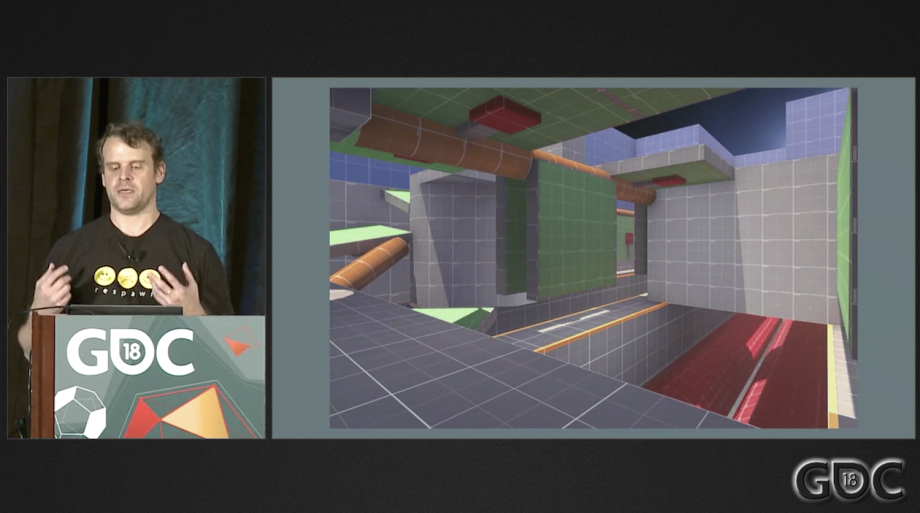
\includegraphics[width=0.85\textwidth]{action_blocks_3}
\caption{Грейбокс-уровень Titanfall 2 в редакторе: простые формы
определяют геометрию боевого пространства до добавления арта.
\textit{Источник: 80.lv / GDC Vault}}
\label{fig:greybox_example}
\end{figure}

\section{Правила грейбоксинга}

\begin{enumerate}[leftmargin=*]
  \item \textbf{Метрики движения}~--- прежде чем строить что-либо,
    определите базовые размеры:

\begin{table}[H]
\centering
\caption{Типичные метрики для Action FPS (UE5 units)}
\begin{tabular}{@{}lcc@{}}
\toprule
\textbf{Параметр} & \textbf{Мин. размер} & \textbf{Комфорт} \\
\midrule
Дверной проём (ширина) & 120 uu & 160 uu \\
Дверной проём (высота) & 200 uu & 220 uu \\
Коридор (ширина) & 200 uu & 300 uu \\
Высота прыжка & 120 uu & -- \\
Дальность double jump & 240 uu & -- \\
Мин. ширина wallrun surface & 50 uu & 100 uu \\
Высота полного укрытия & 180 uu & 200 uu \\
Высота половинного укрытия & 90 uu & 100 uu \\
\bottomrule
\end{tabular}
\end{table}

  \item \textbf{Цветовое кодирование}~--- используйте цвета материалов
    для обозначения функции:
    \begin{itemize}
      \item Серый~--- обычная геометрия
      \item Синий~--- wallrun поверхность
      \item Зелёный~--- безопасная зона / ресурсы
      \item Красный~--- опасная зона / killzone
      \item Жёлтый~--- интерактивные элементы
    \end{itemize}

  \item \textbf{Тестируйте движение первым}~--- прежде чем добавлять
    врагов, убедитесь, что traversal работает и ощущается хорошо

  \item \textbf{Враги~--- последними}~--- геометрия определяет бой,
    не наоборот. Сначала пространство, потом враги
\end{enumerate}


% =============================================================================
% CHAPTER 12: CHECKLIST
% =============================================================================
\chapter{Чек-листы для дизайнера}

\section{Чек-лист: Арена}

\begin{table}[H]
\centering
\begin{tabularx}{\textwidth}{@{}cX@{}}
\toprule
$\square$ & Арена имеет минимум 2 петли (обходных пути) \\
$\square$ & Есть вертикальность (минимум 2 уровня высоты) \\
$\square$ & Ни одна позиция не контролирует всю арену \\
$\square$ & Вход не является лучшей боевой позицией \\
$\square$ & Есть укрытия нескольких типов \\
$\square$ & Есть wallrun-поверхности или dash-маршруты \\
$\square$ & Ресурсы распределены для поощрения движения \\
$\square$ & Арена трансформируется хотя бы 1 раз \\
$\square$ & Есть чёткие spawn points для врагов \\
$\square$ & Тестирована на всех типах апгрейдов игрока \\
\bottomrule
\end{tabularx}
\end{table}

\section{Чек-лист: Энкаунтер}

\begin{table}[H]
\centering
\begin{tabularx}{\textwidth}{@{}cX@{}}
\toprule
$\square$ & Начало: игрок может осмотреть арену до боя \\
$\square$ & Палитра врагов: Aggressor + Anchor + Disruptor \\
$\square$ & Не более 3 типов врагов одновременно \\
$\square$ & Есть эскалация (минимум 2 волны) \\
$\square$ & Есть чёткий момент победы \\
$\square$ & Сложность соответствует месту в кривой пейсинга \\
$\square$ & Энкаунтер проходим без апгрейдов из open world \\
$\square$ & Апгрейды дают ощутимое преимущество \\
\bottomrule
\end{tabularx}
\end{table}

\section{Чек-лист: Пейсинг уровня}

\begin{table}[H]
\centering
\begin{tabularx}{\textwidth}{@{}cX@{}}
\toprule
$\square$ & После каждого боя есть зона отдыха \\
$\square$ & Зоны отдыха разного типа (traversal, лор, puzzles) \\
$\square$ & Интенсивность в целом растёт к финалу \\
$\square$ & Climax Arena~--- самый интенсивный момент \\
$\square$ & Есть resolution (спад) после кульминации \\
$\square$ & Никакие два последовательных сегмента не одинаковы \\
$\square$ & Общий хронометраж: 15--20 минут (с exploration) \\
\bottomrule
\end{tabularx}
\end{table}

\section{Чек-лист: Открытая зона}

\begin{table}[H]
\centering
\begin{tabularx}{\textwidth}{@{}cX@{}}
\toprule
$\square$ & Climax Arena видна из любой точки зоны \\
$\square$ & Прямой путь к Climax Arena всегда доступен \\
$\square$ & Каждая POI даёт уникальную награду \\
$\square$ & POI находятся на расстоянии 1--3 мин друг от друга \\
$\square$ & Навигация интуитивна (weenies, цвет, рельеф) \\
$\square$ & 5--10 POI разных типов \\
$\square$ & Exploration не обязательна, но вознаграждается \\
$\square$ & Апгрейды расширяют toolkit, не числа \\
\bottomrule
\end{tabularx}
\end{table}


% =============================================================================
% CHAPTER 13: REFERENCE GAMES
% =============================================================================
\chapter{Референсные игры и материалы}

\section{Обязательные к изучению}

\begin{table}[H]
\centering
\caption{Ключевые референсы для каждого аспекта}
\begin{tabularx}{\textwidth}{@{}lXX@{}}
\toprule
\textbf{Аспект} & \textbf{Игра} & \textbf{Что изучать} \\
\midrule
Handcrafted levels & Titanfall 2 & Action Blocks, level gimmicks \\
Arena combat flow & DOOM Eternal & Skate parks, push-forward \\
Skill expression & ULTRAKILL & Style system, weapon combos \\
Movement design & Titanfall 2 & Wallrun, momentum, traversal \\
Set-pieces & Titanfall 2 & Effect \& Cause, Into the Abyss \\
Ranking system & ULTRAKILL & P/S/A/B/C/D ranks \\
Compact worlds & Metroid Prime & Interconnected zones, backtracking \\
Encounter design & DOOM 2016 & Enemy triads, resource pressure \\
Environmental puzzle & Half-Life 2 & Physics puzzles, Gravity Gun \\
Open zone design & DOOM Eternal & Hub levels (Fortress of Doom) \\
\bottomrule
\end{tabularx}
\end{table}

\section{Материалы для дальнейшего изучения}

\begin{enumerate}[leftmargin=*]
  \item \textbf{GDC 2018}: <<Designing Unforgettable Titanfall Single Player
    Levels with Action Blocks>> --- Christopher Dionne (бесплатно на YouTube)
  \item \textbf{The Level Design Book} ---
    \url{https://book.leveldesignbook.com/} (бесплатно)
  \item \textbf{Game Developer}: <<A close analysis of Titanfall 2's
    level Effect and Cause>> --- подробный разбор уровня
  \item \textbf{Mapcore}: <<Effect and Cause --- Titanfall 2 Level
    Breakdown>> --- детальный анализ энкаунтеров
  \item \textbf{David Shaver Portfolio}: <<Into the Abyss>> ---
    дизайнерский портфолио с описанием процесса
  \item \textbf{Fullbright}: <<Basics of Effective FPS Encounter Design
    via F.E.A.R.>> --- основы дизайна энкаунтеров
  \item \textbf{Hullett \& Whitehead}: <<Design Patterns in FPS Levels>> ---
    академическая статья о паттернах уровней
\end{enumerate}

\vspace{1cm}

\begin{center}
\begin{tikzpicture}
  \fill[titandark, rounded corners=4pt] (0,0) rectangle (12,2);
  \node[text=white, font=\Large\bfseries] at (6,1.3) {POLARITY};
  \node[text=titanlight, font=\small] at (6,0.6) {Level Design Guide --- Internal Document --- 2026};
\end{tikzpicture}
\end{center}

\end{document}
